\chapter{Vorgehensweise}\label{chap:Vorgehensweise}
Um dem im Kapitel \glqq{}\ref{chap:Motivation} Motivation\grqq{} formulierten Ziel zu folgen, muss zunächst eine Datenquelle gewählt werden.
Anschließend werden deren Daten in eine nutzbare Form übertragen.
Schlussendlich können die Informationen aus den Daten verknüpft, interpretiert und graphisch dargestellt werden.

Der entsprechende Programmcode findet sich in den Programmdateien im Anhang der Bachelorarbeit. \todo{Wo sind die Programmdateien}

Diese Bachelorarbeit basiert teilweise auf den Vorleistungen des Bachelorprojekts von Leander Marius Bürkin.
Ziel dieses Bachelorprojekts war eine Reihe an Deutschlandkarten in einem Video zusammenzufassen, welches die Ausbreitung der COVID-19 Pandemie in Deutschland vom ersten März 2020 bis zum letzten Tag, für den die API des Robert-Koch-Instituts Daten liefert, darstellt.
Das fertige Videos ist verfügbar unter \todo{Video verlinken}.

\section{Datenquellen - Ursprung und Abspeicherung}\label{sec:Datenquelle}

Das Bachelorprojekt sowie diese Bachelorarbeit verwenden Informationen zur COVID-19 Pandemie und den geographischen Daten von 412 deutschen Landkreisen. Alle Daten stammen aus dem \glqq{}COVID-19 Datenhub\grqq{} (https://npgeo-corona-npgeo-de.hub.arcgis.com/) oder wurden aus den daher stammenden Daten generiert. Diese Datenquelle wurde gewählt, weil sie vom Robert-Koch-Institut (RKI, www.rki.de) und dem deutschen Staat referenziert wird.

\todo{wie verlinke ich die URL korrekt?}

\todo{Staat refernzieren}

Insgesamt werden drei verschiedene Datenpakete der API verwendet, zum einen die geographischen Daten der Landkreise, zum anderen die Summe aller aufgetretenen COVID-19 Fälle seit Beginn der Pandemie für jeden Landkreis und jeden Tag seit dem 01.März 2020 sowie eine Auflistung aller Meldungen der Gesundheitsämter, in welchen das  Referenzdatum, das Meldedatum, die Anzahl der betroffenen Menschen und deren tragisches Schicksal (entweder genesen, verstorben oder noch infektiös) angegeben werden. Das Referenzdatum kann als Tag der Infektion interpretiert werden, das Meldedatum als Genesungsdatum beziehungsweise Sterbedatum.

\todo{RKI Paper verlinken}

Die Landkreise, welche das RKI angibt stimmen nicht mit den Landkreisen des Statistischen Bundesamtes überein: In den Daten des RKIs gibt es 118 Landkreise mehr, beziehungsweise wenn man die kreisfreien Städte abzieht, zwölf Landkreise mehr. Diese Diskrepanz kommt durch die Aufteilung von Berlin in seine 12 Bezirke und Eisenach wird in den Daten des RKIs als eigene kreisfreie Stadt gewertet und nicht zum Wartburgkreis hinzugezählt, der Stadtkreis Eisenach ist mit dem Gemeindeschlüssel 16056 versehen. Trotz dieser Unterschiede und obwohl auch kreisfreie Städte miteinbegriffen sind, wird nach Vorbild des RKIs im folgenden der Begriff \glqq{}Landkreise\grqq{} für alle 412 Gebiete verwendet.
\todo{Verlinken: https://www.destatis.de/DE/Themen/Laender-Regionen/Regionales/Gemeindeverzeichnis/Administrativ/03-regierungsbezirke.html}
\todo{https://www.destatis.de/DE/Themen/Laender-Regionen/Regionales/Gemeindeverzeichnis/Administrativ/04-kreise.html}
\todo{Liste der NUTS-Codes Gemeindeschlüssel leiten sich daraus ab. URL siehe Kommentar}
%https://eur-lex.europa.eu/legal-content/DE/TXT/PDF/?uri=CELEX:32016R2066&from=EN
Die Daten werden abgespeichert, damit nicht bei jeder Ausführung eine zeitaufwendige Anfrage an die API zu stellen und die Daten aufzubereiten.

Bevor die deutschen Landkreise gewählt wurden, wurden die COVID-19 Daten der USA verwendet. Jedoch wieß die API, die die Daten der John Hoppkins Universität bereitstellte, einige Fehler auf und wurde schlussendlich entfernt.
Dieser Umstand findet seine Auswirkungen immernoch in einigen Begriffen im Programmcode (bspw. \glqq{}county\grqq{} für Landkreis und \glqq{}district\grqq{} für Regierungsbezirk).
\todo{Tauchen "counties" etc. anderstwo noch auf?}

\section{Datenaufbereitung}
Bevor die Daten genutzt werden können müssen sie gecheckt werden, überflüssige Informationen entfernt werden und neue Kennzahlen aus den gegebenen Informationen berechnet werden. Daten vor der Datenaufbereitung, welche direkt von der API oder einem Backup davon stammen, werden als \glqq{}unmodifizierte\grqq{} Daten bezeichnet. 

Daten, die rudimentär auf Vollständigkeit überprüft wurden, aus den Daten generierte Daten enthalten und bei welchen überflüssige Informationen entfernt wurden, werden \glqq{}modifizierte\grqq{} Daten genannt.

Zunächst werden die unmodifizierten Daten in eine übersichtlichere Form übertragen und es wird sichergestellt, dass gleich viel Werte für jeden Landkreis vorhanden sind. Zudem werden die Umrisse der circa 100 Landkreise von Hand geprüft, welche mehrere Polygone enthalten, diese werden entweder als Ausschnitt oder als reale Fläche interpretiert.

Nachdem die unmodifizierten Daten in eine übersichtlichere Form übertragen und überprüft wurde werden aus den Daten weitere Werte berechnet.

Die Bevölkerungsdichte wird berechnet, indem die Anzahl der Einwohner durch die Fläche in Quadratmetern geteilt wird. Beide Informationen werden von der API bereitgestellt.
Die Bevölkerungsdichte wird auch für die Regierungsbezirke berechnet. Nicht alle Bundesländer wurden in Regierungsbezirke unterteilt, in diesem Fall wird die Bevölkerungsdichte des Bundeslandes gewählt. Im folgenden wird dennoch von \glqq{}den Regierungsbezirken\grqq{} gesprochen. 
% Zudem sind die Stadtstaaten Bremen und Hamburg zum Regierungsbezirk Lüneburg hinzugefügt und der Stadtstaat Berlin zum Bundesland Brandenburg hinzugefügt. Die Regierungsbezirke werden durch die ersten zwei beziehungsweise drei Ziffern des Gemeindeschlüssel herausgefiltert.
Sowohl die Bevölkerungsdichten der Landkreise wie auch die Bevölkerungsdichten der Regierungsbezirke werden zur Einordnung der Korrelationsanalysen auf einer Deutschlandkarte dargestellt, wobei die Farbe die Bevölkerunsdichte repräsentiert, wie in \autoref{sec:Durchschnitt, Farbgebung und Skalierung} beschrieben.

Die sieben Tages Inzidenz wird für jeden Tag seit Beginn der Pandemie berechnet. Hierfür wird die akkumulierte Zahl der Fälle am siebten Tag vor dem jeweiligen Tag von der akkumulierte Zahl der Fälle am jeweiligen Tag abgezogen, dies ergibt die neu hinzugekommenen Fälle innerhalb von sieben Tagen.
Diese Zahl wird durch die Anzahl der Bewohner des Landkreises geteilt und mit 100.000 multipliziert. Dadurch werden die Werte der einzelnen Landkreise vergleichbar.

\todo{sieben Tages Inzidenz Quelle angeben}

Um die Auflistung aller Meldungen der Gesundheitsämter nutzen zu können, müssen diese erst für jeden Landkreis und jeden Tag gesammelt und aufsummiert werden:
Das Referenzdatum wird als Tag der Infektion interpretiert. Die Anzahl der betroffenen Individuen wird für jeden folgenden Tag zur akkumulierten Anzahl der Fälle hinzuaddiert.
Das Meldedatum wird als Tag der Genesung beziehungsweise Tag des Todes interpretiert, je nachdem ob die Meldung Genesung oder Tod angibt. Die Anzahl der betroffenen Individuen wird hier zum einen für jeden folgenden Tag zur akkumulierten Anzahl der Genesenen/Verstorbenen hinzuaddiert. Zum anderen wird die Anzahl der betroffenen Individuen für jeden Tag zwischen dem Referenzdatum und dem Meldedatum zu den aktiven Fällen hinzuaddiert.

Mithilfe der Gesamtbevölkerung eines Landkreises werden aus diesen Daten für jeden Tag und jeden Landkreis alle drei Kategorien des SIR-Modells berechnet:

\begin{itemize}
    \item \glqq{}susceptible\grqq{}: Die Gesamtbevölkerung des Landkreises minus die akkumulierte Anzahl der Fälle.
    \item \glqq{}infectious\grqq{}: Liegt als aktive Fälle bereits vor.
    \item \glqq{}recovered\grqq{}:
    Die Summe aus der akkumulierten Anzahl der Genesenen und der Verstorbenen. Oder die akkumulierte Anzahl der Fälle minus die aktiven Fälle, solange zu jeder Meldung ein Referenzdatum angegeben ist, entspricht dies der ersten Variante.
\end{itemize}

Um ein Gefühl dafür zu bekommen, welcher Lankreis wie hart von der Corona Pandemie betroffen ist, wird die akkumulierte Anzahl der COVID-19 Fälle des letzten Tages durch die Bevölkerung des Landkreises geteilt und farblich in einer Deutschlandkarte dargestellt.

\section{Datenformat}
Die Daten liegen in einer Kombination aus sogenannten Python Dictionaries und sogennanten Python Listen vor.

Ein Dictionary ist dadurch charakterisiert, dass man über den Namen eines Elements (der \glqq{}Key\grqq{}) das Element (das \glqq{}Value\grqq{}) bekommt, ähnlich wie man früher in Telefonbüchern anhand des Namens (der Key) die Telefonnummer (das Value) erhalten hat.
\todo{soll ich die Fachbegriffe hinzufügen? Werden sie überhaupt benutzt?}

Listen sind dadurch charakterisiert, dass sie Elemente in einer fixen Reihenfolge enthalten und sich diese durch ihren Index leicht auffindbar machen. So sind beispielsweise die Anzahl der COVID-19 Fälle der einzelnen Tage chronologisch in einer Liste gespeichert, sodass man daraus direkt eine Abbildung erstellen kann.


Die Programmdateien erstellen drei verschiedene sogenannte globale Dictionaries, welche (in untergeordneten Dictionaries und Listen) alle Daten enthalten. Globale Dictionaries sind in allen Dateien verfügbar und unterscheiden sich insofern von lokalen Dictionaries/Listen, welche nur in einzelnen Programmabschnitten vorliegen und daher nicht derart zentral sind.
Die drei Dictionaries heißen\todo{vervollständigen, districts}
\begin{itemize}
    \item covid19
    \item counties\_geography
    \item non\_county\_specific\_data
\end{itemize}

\textbf{covid19}\\
Das Dictionary covid19 speichert die COVID-19 Fälle jedes deutschen Landkreises und die daraus berechnete sieben Tages Inzidenz.

Mit dem Gemeindeschlüssel eines Landkreises als Key und dem zusätzlichen Key \glqq{}cases\grqq{} erhält man die akkumulierte Anzahl an COVID-19 Fällen pro Tag des Landkreises als Liste.

Mit dem Gemeindeschlüssel eines Landkreises als Key und dem Key \glqq{}incidences\grqq{} erhält man die sieben Tages Inzidenz pro Tag des Landkreises als Liste.

Beide Listen enthalten für jeden Tag seit dem 01.03.2020 bis zu dem Tag der aktuellsten Daten jeweils einen Eintrag.

Die Anzahl an COVID-19 Fällen pro Tag stammt aus dem \glqq{}COVID-19 Datenhub\grqq{}. Die sieben Tages Inzidenz wird wie in \autoref{sec:Datenaufbereitung} beschrieben aus den Daten vom COVID-19 Datenhub berechnet.

\textbf{counties\_geography}\\
Das Dictionary counties\_geography enthält zu jedem Landkreis ein Dictionary mit den folgenden Elemente:
\begin{itemize}
    \item[name:] Der Name des Landkreises
    \item[population:] Die Einwohnerzahl des Landkreis aus einer offiziellen Schätzung (nähere Informationen finden sich im COVID-19 Datenhub). Diese Zahlen werden auch für die offizielle Berechnung der sieben Tages Inzidenz verwendet.
    \item[area\_in\_m2:] Die Fläche des Landkreises in Quadratmetern
    \item[geometry:] Die Form des Landkreises in einer für die Darstellung angepassten Form
    \item[raw\_geometry:] Die Form des Landkreises in der originalen Form
    \item[population\_density:] Die Bevölkerungsdichte des Landkreises, berechnet aus der Fläche des Landkreises und seiner Einwohnerzahl
\end{itemize}
Außer die Bevölkerungsdichte, welche berechnet wird, und die angepassten Formen der Landkreise, welche aus den origialen Formen generiert werden, stammen alle Daten direkt aus dem \glqq{}COVID-19 Datenhub\grqq{}.

\textbf{non\_county\_specific\_data}
Das Dictionary non\_county\_specific\_data enthält die folgenden Elemente:
\begin{itemize}
    \item[unixtime:] Die Unixzeit, wie sie vom COVID-19 Datenhub zur Verfügung gestellt wird: Die Zahl der Millisekunden seit dem 01.01.1970 00:00 Uhr UTC. Die Zahl der COVID-19 Fälle und die sieben Tages Inzidenz eines entsprechenden Tages befinden sich an der selben Stelle in Ihrer jeweiligen Liste, wie der Tag in dieser Liste.
    \item[states:] Die Name und Nummern der deutschen Bundesländer. Die ersten beiden oder die erste Zahl des Gemeindeschlüssel eines Landkreises geben das Bundesland an, in welchem der Landkreis liegt. Die ersten zwei bzw. drei Zahlen geben den Regierungsbezirk an, in dem der Landkreis. Sollte es im jeweiligen Bundesland keine Regierungsbezirke geben, entspricht dies dem Bundesland.
    \item[highest\_case\_number:] Die höchste akkumulierte Fallzahl unter allen Landkreisen.
    \item[lowest\_case\_number:] Die niedrigste akkumulierte Fallzahl unter allen Landkreisen.
    \item[highest\_incidence:] Die höchste sieben Tages Inzidenz eines Tages unter allen Landkreisen.
    \item[lowest\_incidence:] Die niedrigste sieben Tages Inzidenz eines Tages unter allen Landkreisen.
    \item[UTC:] Die Unixzeit konvertiert in die Koordinierte Weltzeit \glqq{}DD.MM.YYYY\grqq{}.
    \item[UTC+7days:] Die Liste der Zeiten gespeichert in UTC plus sieben Tage vor dem erstem Datum in der Liste, um den Zeitraum der sieben Tages Inzidenz der ersten sieben Tage darstellen zu können: die hierfür verwendeten Zeiträume beginnen jeweils vor dem ersten hier dokumentierten Fall.
\end{itemize}
Die Unixzeit, die Namen und die Nummern der Bundesländer stammen aus dem \glqq{}COVID-19 Datenhub\grqq{}. Alle anderen Informationen wurden gesammelt oder berechnet.

In Abbildung \ref{fig:dicts_als_code} sind die drei Dictionaries dargestellt, wie sie auch im Programm verwendet werden.
\begin{figure}[H]
    \centering
    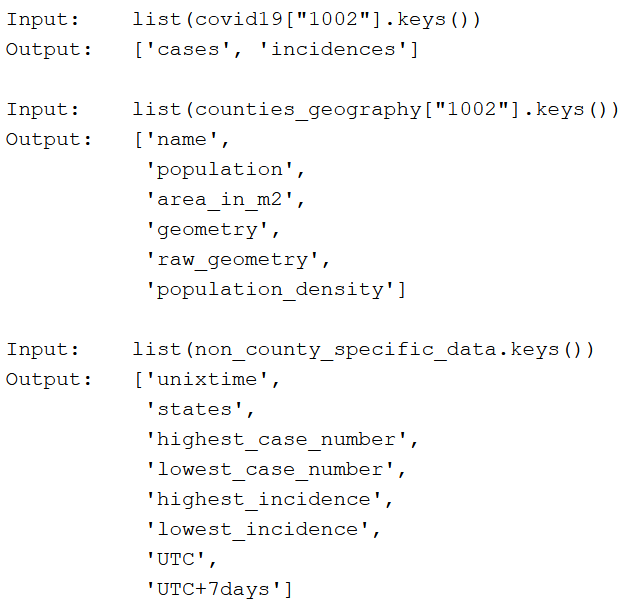
\includegraphics[width=0.8\textwidth]{figures/Vorgehensweise/Dictionarys Bachelorprojekt.png}
    \caption{
    Die Dictionaries non\_county\_specific\_data, counties\_geography und covid19 mit ihren jeweiligen Schlüsseln.
    Für die Dictionaries covid19 und counties\_geography wurde jeweils der Landkreis Kiel (Gemeindeschlüssel 1002) zur Veranschaulichung verwendet.}
    \label{fig:dicts_als_code}
\end{figure}

\todo{Daten aus Meldungen einpflegen}
\section{Datendarstellung}
Zuerst werden die Daten der Landkreise und Regierungsbezirke dargestellt, welche auf einfachen Gleichungen beruhen und lediglich zur Einordnung der anderen Ergebnisse dienen:
\begin{itemize}
    \item Die Bevölkerungsdichte, um schlussfolgerungen ziehen zu können, ob diese in irgendeinerweise mit dem Infektionsverhalten zusammenhängt
    \item Die Anordnung der Gebiete, wenn man sie nach ihrem Gemeindeschlüssel sortiert - Die Sortierung erfolgt hier lexikographisch, das heißt, das die Länge des Gemeindeschlüssels keine Rolle spielt, sondern immer das erste Zeichen verglichen wird und bei Übereinstimmung das nächste (Dadurch ergibt sich eine einheitlichere Nord-Süd-Aufteilung als die Sortierung nach der Größe)
    \item Die Summe der 7-Tages Inzidenzen als Maß wie stark ein Gebiet betroffen war
\end{itemize}
\subsection{SIR-Modell}
Da die Zahl der aktiven Fälle sehr niedrig und dementsprechend sensibel gegenüber kleinen Anomalien, ist, wird nur auf Bundesebene ein SIR-Modell erstellt und dargestellt. 
Hierfür werden die drei Kennzahlen des SIR-Modells in drei Abbildungen dargestellt.
\todo{SIR-Modell einfügen und mit Grundlagen abgleichen}

\subsection{Korrelationsanalyse}
Insgesamt werden folgende verschiedene Arten von Korrelationsanalysen durchgeführt:
\begin{itemize}
    \item Die Korrelation einzelner Stadtkreise welche komplett von einem Landkreis umgeben sind.
    \item Die Korrelation aller Landkreise untereinander sortiert nach Bevölerungsdichte.
    \item Die Korrelation aller Regierungsbezirke untereinander sortiert nach Bevölerungsdichte.
    \item Die Korrelation aller Landkreise untereinander sortiert nach dem Gemeindeschlüssel, entspricht einer groben Nord-Süd Aufteilung.
    \item Die Korrelation aller Regierungsbezirke untereinander sortiert nach dem Gemeindeschlüssel, entspricht einer groben Nord-Süd Aufteilung.
\end{itemize}
Es wird jeweils die Korrelation zwischen den Zeitserien der 7 Tages Inzidenzen nach den in \autoref{sec:BeschreibungKorrelationsanalyse} beschriebenen Methoden untersucht. Hieraus ergibt sich jeweils eine Liste an Werten, welche angeben, bei welchem zeitlichen Versatz wie wahrscheinlich eine Korrelation vorliegt.

Um dieses Verfahren zum Einstieg übersichtlich darzustellen, werden zuerst die Korrelationen zwischen den Landkreisen aus Tabelle \ref{tab:landkreise_um_städte} und den Stadtkreisen, die sie umgeben, berechnet. An ihnen lässt sich besonders gut testen, ob sich in den Korrelationswahrscheinlichkeiten zwischen einer Stadt und ihrem Umland eine zeitliche Verschiebung feststellen lässt.

In \autoref{fig:selected_counties} sind die ausgewählten Landkreise mit den Stadtkreisen, die sie umgeben abbgebildet.
\begin{table}[H]
    \centering
    \begin{tabular}{c|c|c|c}
    Name des Land-&AGS &Umgebener  &AGS\\
    kreises (LK)  &Landkreis&Stadtkreis (SK)&Stadtkreis\\
    \hline
Kassel & 6633 & Kassel & 6611 \\\hdashline
Trier-Saarburg & 7235 & Trier & 7211 \\\hdashline
Südliche Weinstraße & 7337 & Landau i.d.Pfalz & 7313 \\\hdashline
Südwestpfalz & 7340 & Pirmasens & 7317 \\\hdashline
Heilbronn & 8125 & Heilbronn & 8121 \\\hdashline
Rastatt & 8216 & Baden-Baden & 8211 \\\hdashline
Rosenheim & 9187 & Rosenheim & 9163 \\\hdashline
Landshut & 9274 & Landshut & 9261 \\\hdashline
Straubing-Bogen & 9278 & Straubing & 9263 \\\hdashline
Amberg-Sulzbach & 9371 & Amberg & 9361 \\\hdashline
Neustadt a.d.Waldnaab & 9374 & Weiden i.d.OPf & 9363 \\\hdashline
Regensburg & 9375 & Regensburg & 9362 \\\hdashline
Bamberg & 9471 & Bamberg & 9461 \\\hdashline
\begin{comment}
Bayreuth & 9472 &  &  \\\hdashline
Coburg & 9473 &  &  \\\hdashline
Hof & 9475 &  &  \\\hdashline
Ansbach & 9571 &  &  \\\hdashline
Schweinfurt & 9678 &  &  \\\hdashline
Würzburg & 9679 &  &  \\\hdashline
Ostallgäu & 9777 &  &  \\\hdashline
\end{comment}
Oberallgäu & 9780 & Kempten & 9763 \\\hdashline
Potsdam-Mittelmark & 12069 & Brandenburg a.d. Havel & 12051 \\\hdashline
Spree-Neiße & 12071 & Cottbus & 12052 \\\hdashline
Saalekreis & 15088 & Halle (Saale) & 15002 \\\hdashline
Weimarer Land & 16071 & Weimar & 16055
    \end{tabular}
    \caption{Landkreise mit Name und Gemeindeschlüssel (AGS), die den jeweils mit Name und Gemeindeschlüssel gekennzeichneten Stadtkreis komplett umgeben.}
    \label{tab:landkreise_um_städte}
\end{table}

\begin{figure}[H]
    \centering
    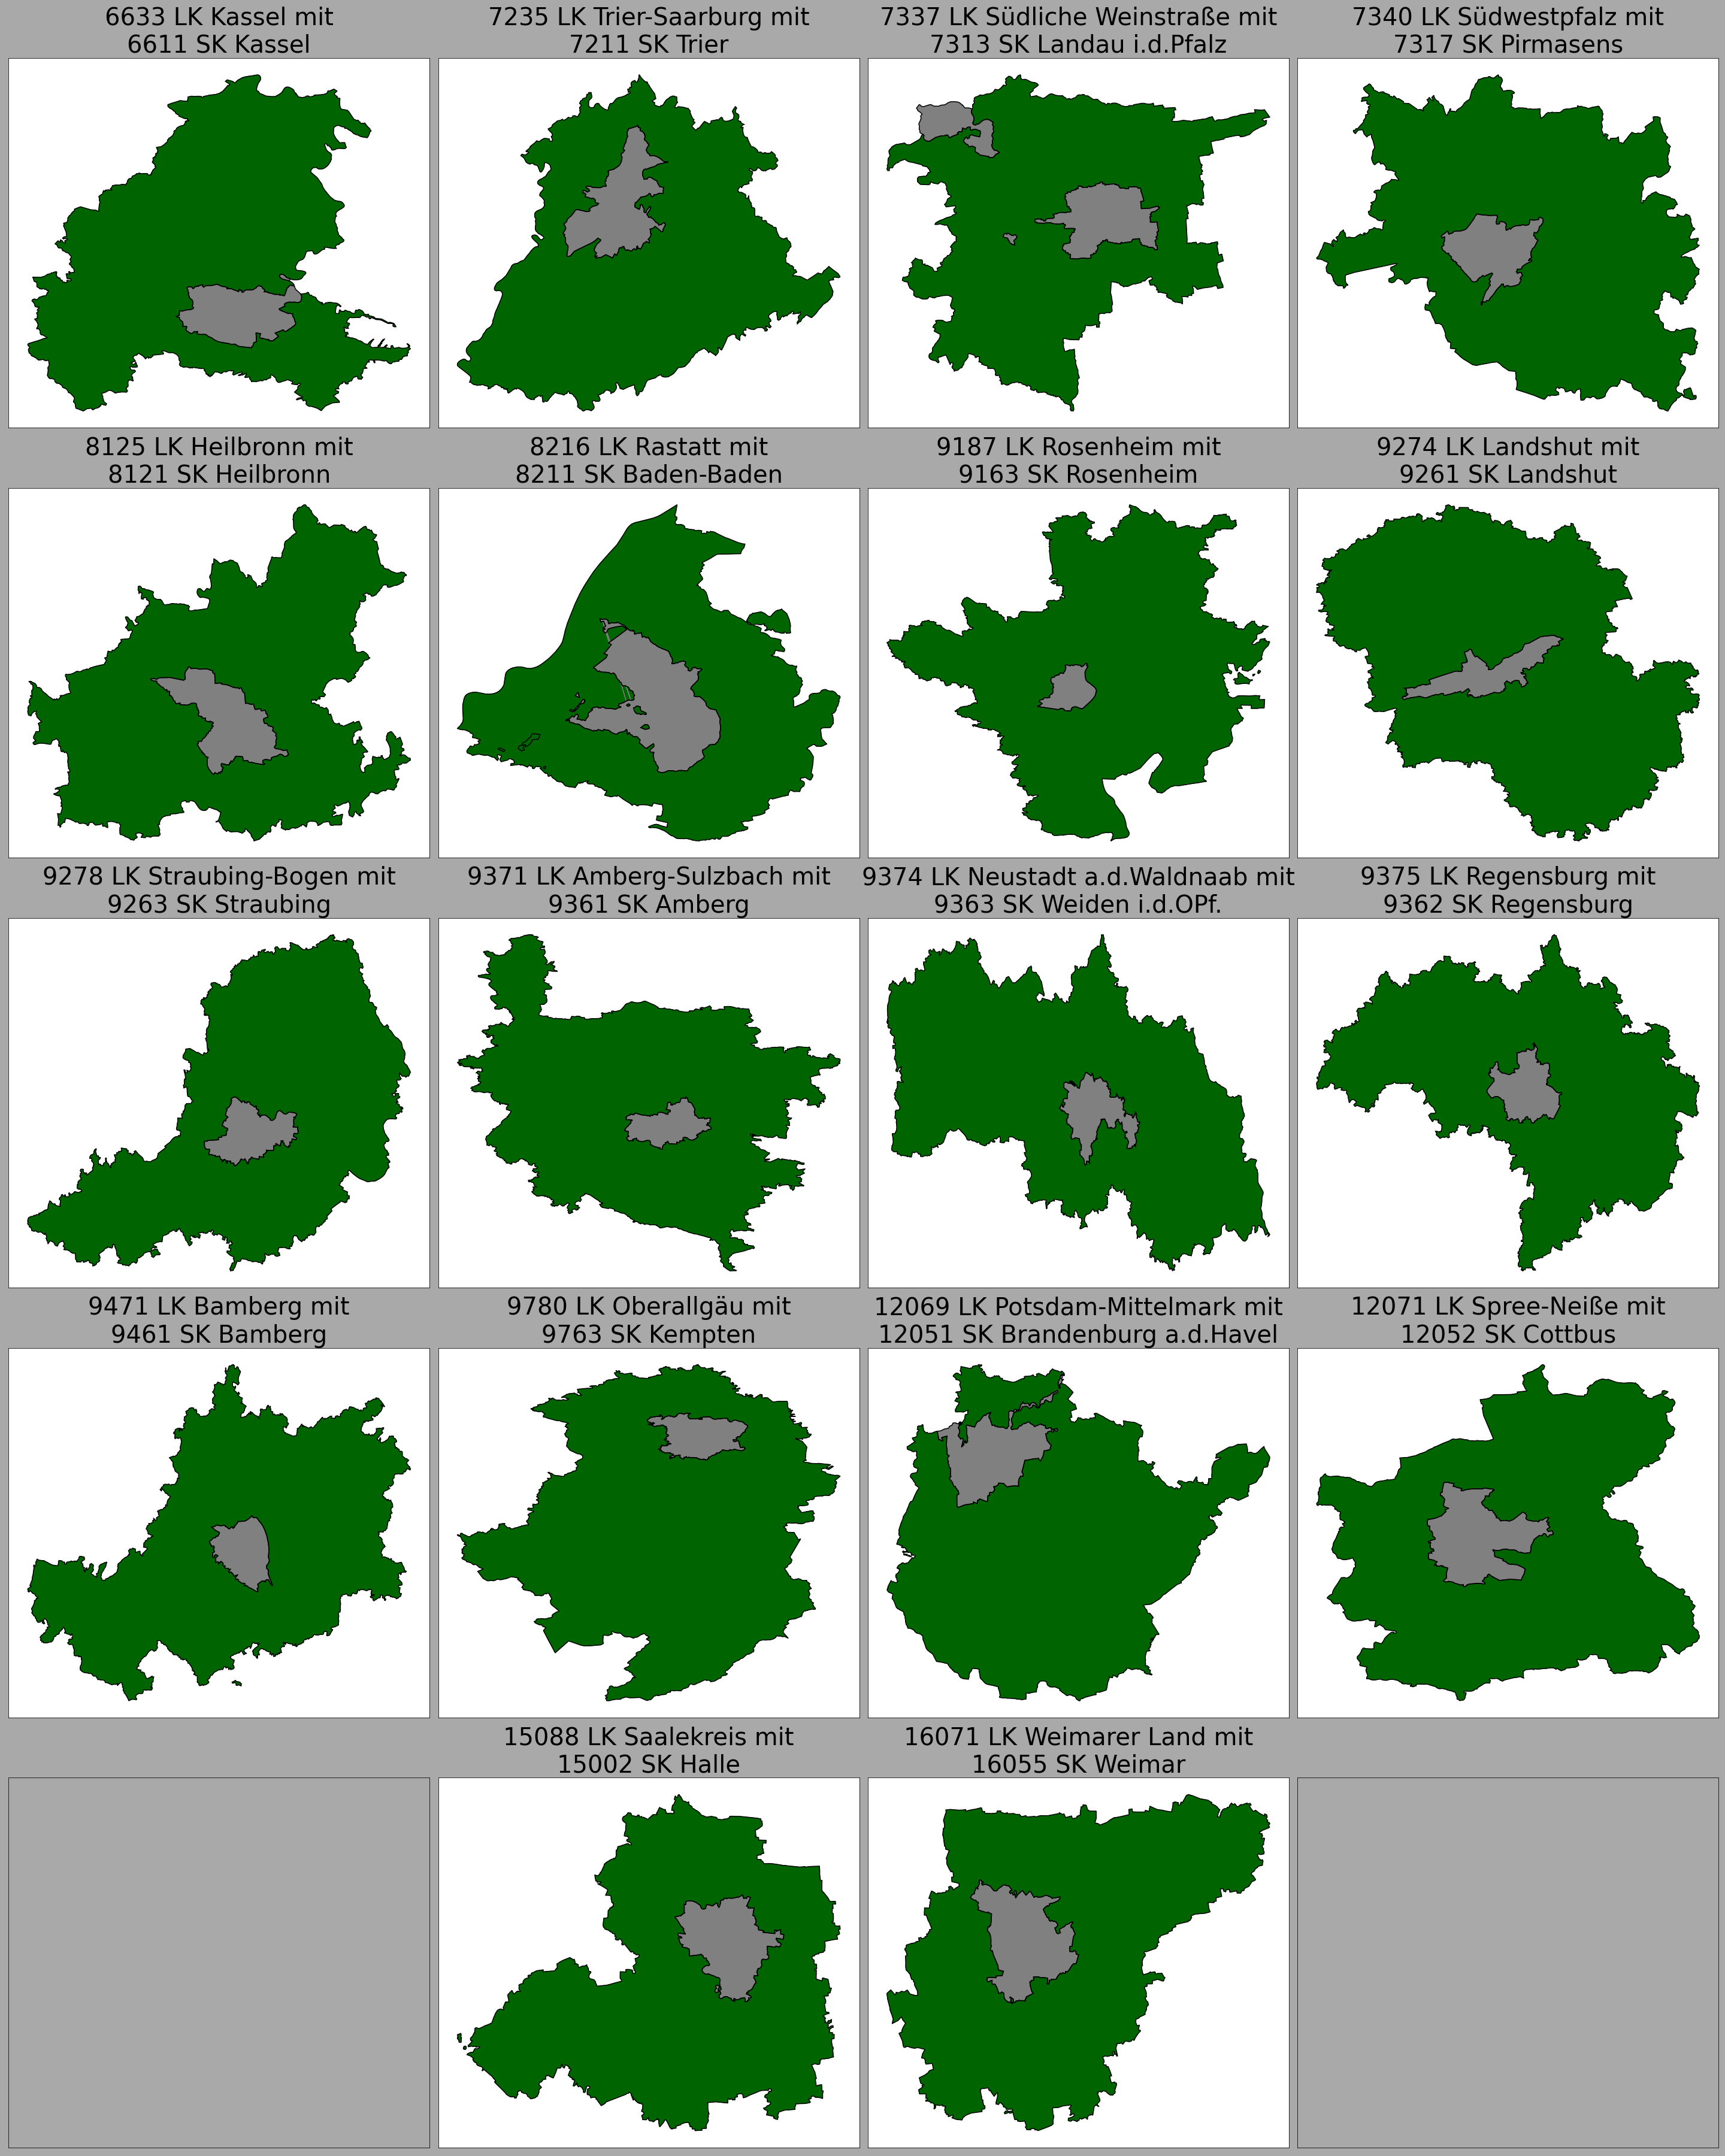
\includegraphics[width=\textwidth]{figures/Vorgehensweise/selected_counties.png}
    \caption{Die ausgewählten Landkreise mit den Stadtkreisen, die sie jeweils umgeben.}
    \label{fig:selected_counties}
\end{figure}

\subsubsection{Matrix der maximalen Wahrscheinlichkeiten}
Um die Korrelationswahrscheinlichkeiten aller Landkreise/Regierungsbezirke untereinander darzustellen, werden aus den Korrelationswahrscheinlichkeiten zwei Werte berechnet, wie zwei Landkreise/Regierungsbezirke in Relation zueinander stehen könnten.

Zum einen werden die Verschiebungen mit der höchsten Wahrscheinlichkeit in eine Matrix eingetragen, wobei jede Zeile und Spalte einem Landkreis/Regierungsbezirk zugeordnet ist.

Der Eintrag in einer Zelle entspricht der wahrscheinlichsten zeitlichen Verschiebung des Verlaufs der 7 Tages Inzidenz des Landkreises/Regierungsbezirkes der Spalte im Vergleich zu dem Verlauf der 7 Tages Inzidenz des Landkreises/Regierungsbezirkes der Zeile.
Somit ist die Matrix symmetrisch an der Diagonalen von links oben nach rechts unten, lediglich die Vorzeichen unterscheiden sich. Die Diagonale ist mit Nullen besetzt, da die Korrelationswahrscheinlichkeit zu sich selbst trivialerweise bei einer Verschiebung von $\tau=0$ am größten ist, da die Werte und Trends komplett identisch sind.

Summiert man die Werte einer Zeile auf und teilt sie durch die Anzahl der Werte, erhält man die Anzahl der Tage, die die sieben Tages Inzidenz des Landkreises, der dieser Zeile zugeordnet ist, im Durchschnitt zu den 7 Tages Inzidenzen aller anderen deutschen Landkreisen versetzt ist.
Somit lässt sich farblich auf einer Deutschlandkarte eine sehr grobe Darstellung erzeugen, welche Landkreise im Schnitt wieviel früher einen Anstieg der 7 Tages Inzidenzen aufwiesen.

\subsubsection{Matrix der aufsummierten Wahrscheinlichkeiten}
Bei der zweiten Möglichkeit werden die Wahrscheinlichkeiten für alle positiven zeitlichen Verschiebungen zusammenaddiert und die Wahrscheinlichkeiten für alle negativen zeitlichen Verschiebungen davon abgezogen, 
um die kompletten Informationen aus der Liste an Korrelationswahrscheinlichkeiten zu verarbeiten und nicht nur einen Wert herauszunehmen. Diese Korrelation kann ebenfalls als Matrix dargestellt werden. In diesem Fall zeigt der Wert einer Zelle, ob die Zahl der COVID-19 Fälle des Landkreises/Regierungsbezirkes der Spalte eher vor oder nach den COVID-19 Fällen des Landkreises/Regierungsbezirkes der Zeile steigen und fallen. Die Information, um wieviele Tage die Kurve wahrscheinlich verschoben ist, geht verloren. Auch diese Matrix ist (mit verkehrtem Vorzeichen) symmetrisch an der Diagonalen von links oben nach rechts unten. Diese Diagonale ist ebenfalls mit Nullen besetzt, da die positive Verschiebung symmetrisch zur negativen Verschiebung ist.

Summiert man die Werte einer Zeile auf, erfährt man wie wahrscheinlich die 7 Tages Inzidenzen des Landkreises/Regierungsbezirks, der der Zeile zugeordnet ist, dem nationalen Schnitt nacheilen oder vorauseilen.
Somit lässt sich farblich auf einer Deutschlandkarte eine sehr grobe Darstellung erzeugen, welche Landkreise im Schnitt früher einen Anstieg der 7 Tages Inzidenzen aufwiesen. Es lässt sich jedoch auch hier keine Aussage mehr darüber treffen, wieviele Tage dieser Versatz vermutlich entspricht.

Da bei einer größeren Verschiebung immer weniger Produkte aufsummiert werden und schlussendlich durch die Anzahl der Produkte geteilt wird, fallen einzelne Ausbrüche stärker ins Gewicht, je größer die Verschiebung ist. Daher werden die Listen mit den Korrelationswahrscheinlichkeiten für die Matrizen für eine maximale Verschiebung von $\tau$ von $-50$~Tage $\leq\tau\leq50$~Tage erstellt. Zudem werden die Matrizen für die maximalen Verschiebungen von $-30$~Tage $\leq\tau\leq30$~Tage und $-14$~Tage $\leq\tau\leq14$~Tage erstellt.

Diese Matrizen werden jeweils mit beiden Methoden für alle Landkreise und alle Regierungsbezirke erstellt.